% File: traffic_control_signals.tex, author: John Sauter,
% date: July 4, 2025.

% Copyright © 2025 by John Sauter.
% Licensed under the Creative Commons Attribution-ShareAlike 4.0 International
% license.  See https://creativecommons.org/license/by-sa/4.0/.

\documentclass[letterpaper,twoside]{article}
\usepackage[capbesideposition=outside,facing=no,capbesidesep=quad]{floatrow}
\usepackage{fontspec}
\usepackage{lmodern}
\usepackage{amsmath}
%\usepackage[english]{babel}
\usepackage{xcolor}
%\usepackage{multicol}
\usepackage{array}
\usepackage{longtable}
\usepackage{enumitem}
\usepackage[super]{nth}
\usepackage{fancyhdr}
\usepackage{xfrac}
\usepackage{fnpct}
\usepackage{siunitx}
\usepackage{graphicx}
\usepackage{natbib}
\usepackage[kpsewhich=true]{minted}
\usepackage[tracking]{microtype}
\usepackage{hyphenat}
\usepackage{fancyvrb}
\usepackage{relsize}
\usepackage{hyperxmp}
%\usepackage{flexisym}
\usepackage{tikz}
\usetikzlibrary {babel}

% Font choices: pick one.

% 1. Latin Modern matches Don Knuth's Computer Modern
% Note that Latin Modern displays U+02BC (Modifier Letter Apostrophe)
% as a space.  This letter is used when naming Mesoamerican
% Long Count dates.
%\usepackage{unicode-math}
%\setmainfont{Latin Modern Roman}[SmallCapsFont={Latin Modern Roman Caps}]
%\setmonofont{Latin Modern Mono}
%\setmathfont{Latin Modern Math}
%\newcommand{\filename}{\ttfamily\smaller}

% 2. Libertine
%\usepackage{unicode-math}
%\setmainfont[Ligatures={Common},Numbers=Proportional]{Linux Libertine O}
%\setsansfont{Linux Biolinum O}
%\setmathfont[Scale=MatchUppercase]{libertinusmath-regular.otf}
%\newcommand{\filename}{\ttfamily}

% 3. Garamond Libre
%\usepackage{unicode-math}
%\usepackage{garamondlibre}
%\newcommand{\filename}{\ttfamily}

% 4. Old Standard
% Small caps doesn't work.
%\usepackage{unicode-math}
%\setmainfont{OldStandard}
%\newcommand{\filename}{\ttfamily}

% 5. Liberation
% Small caps doesn't work.
%\usepackage{unicode-math}
%\defaultfontfeatures{Scale=MatchLowercase}
%\setmainfont{Liberation Serif}
%\setsansfont{Liberation Sans}
%\setmonofont[SmallCapsFont={Liberation Mono}]{Liberation Mono}
%\newcommand{\filename}{\ttfamily}

% 6. GNU Freefont
%\usepackage{unicode-math}
%\setmainfont{FreeSerif}
%\setsansfont{FreeSans}
%\setmonofont{FreeMono}
%\newcommand{\filename}{\ttfamily\smaller}
%\renewcommand\RSpercentTolerance{0}

% 7. Andika
%\usepackage{unicode-math}
%\setmainfont{Andika}
%\newcommand{\filename}{\ttfamily}

% 8. Bahnschrift
%\usepackage{unicode-math}
%\setmainfont{Bahnschrift}
%\newcommand{\filename}{\ttfamily}

% 9. Charis Sil
%\usepackage{unicode-math}
%\setmainfont{Charis Sil}
%\newcommand{\filename}{\ttfamily}

% 10. E B Garamond
%\usepackage{unicode-math}
%\setmainfont{ebgaramond}
%\setsansfont{Charis Sil}
%\setmonofont[SmallCapsFont={Liberation Mono}]{source code pro}
%\setmathfont{Garamond-Math.otf}
%\newcommand{\filename}{\ttfamily\smaller}

% 11. Junicodevf, not yet available in TexLive-2023/Fedora 40 as of
% June 30, 2024.
%\usepackage{unicode-math}
%\usepackage[
%  MainRegularSizeFeatures={
%    {size=8.6,wght=550,wdth=120},
%    {size=10.99,wght=475,wdth=115},
%    {size=21.59,wght=400,wdth=112.5},
%    {size=21.59,wght=351,wdth=100}
%  },
%  MainItalicSizeFeatures={
%    {size=8.6,wght=550,wdth=118},
%    {size=10.99,wght=475,wdth=114},
%    {size=21.59,wght=450,wdth=111},
%    {size=21.59,wght=372,wdth=98}
%  },
%  MainBoldSizeFeatures={
%    {size=8.6,wght=700,wdth=120},
%    {size=10.99,wght=700,wdth=115},
%    {size=21.59,wght=650,wdth=112.5},
%    {size=21.59,wght=600,wdth=100}
%  },
%  MainBoldItalicSizeFeatures={
%    {size=8.6,wght=700,wdth=118},
%    {size=10.99,wght=700,wdth=114},
%    {size=21.59,wght=650,wdth=111},
%    {size=21.59,wght=600,wdth=98}
%  }
%]{junicodevf}
%\newcommand{\filename}{\ttfamily\smaller}

% 12. Lato, not yet available in TexLive-2023/Fedora 40 as of June 1, 2024
%\usepackage[default]{lato}
%\usepackage[default]{lete-sans-math}
%\setsansfont{Lato}[Extension = .ttf,
%  UprigthtFont = *-Regular,
%  BoldFont = *-Bold,
%  ItalicFont = *-Italic,
%  BoldItalicFont = *-BoldItalic]
%\newcommand{\filename}{\ttfamily\smaller}

% 13. New Computer Modern, book weight
\usepackage{unicode-math}
\usepackage{newcomputermodern}
\newcommand{\filename}{\ttfamily\smaller}

\usepackage[pdfencoding=unicode,pagebackref,breaklinks]{hyperref}
\bibliographystyle{plainnat}
\setcitestyle{numbers,square}
% Pages styles
%\setlength{\headheight}{22.5pt}
\pagestyle{fancy}
\fancyhead{}
\fancyhead[LE]{\thepage}
\fancyhead[CE]{{\scshape John Sauter}}
\fancyhead[CO]{{\scshape how traffic control signals work}}
\fancyhead[RO]{\thepage}
\renewcommand{\headrulewidth}{0pt}
\fancyfoot{}
\setlength\tabcolsep{1mm}
\renewcommand\arraystretch{1.3}

\begin{document}
\title{How Traffic Control Signals Work\footnote{Copyright
    {\copyright} 2025 by John Sauter.
    This paper is made available under a
    Creative Commons Attribution-ShareAlike 4.0 International License.
    You can read a human-readable summary of the license at
    \href{https://creativecommons.org/licenses/by-sa/4.0}{https://creativecommons.org/licenses/by-sa/4.0},
    which contains a link to the full text of the license.
    See also section \ref{section:Licensing} of this paper.}
}
\author{John Sauter\footnote{
    System Eyes Computer Store,
    20A Northwest Blvd.  Ste 345,
    Nashua, NH  03063-4066,
    e-mail: John\_Sauter@systemeyescomputerstore.com,
    telephone: (603) 424-1188}}
\hypersetup{unicode=true,
  pdfauthor={John Sauter},
  pdftitle={How Traffic Control Signals Work},
  pdfsubject={traffic control signals},
  pdfkeywords={traffic intersections signals},
  pdfcontactaddress={System Eyes Computer Store, 20A Northwest Blvd.  Ste 345},
  pdfcontactcity={Nashua},
  pdfcontactcountry={USA},
  pdfcontactemail={John\_Sauter@systemeyescomputerstore.com},
  pdfcontactphone={603-424-1188},
  pdfcontactpostcode={03063-4066},
  pdfcontactregion={New Hampshire},
  pdfcontacturl={https://www.systemeyescomputerstore.com},
  pdfcopyright={Copyright {\copyright} 2025 by John Sauter},
  pdfurl={https://www.systemeyescomputerstore.com/traffic\%5Fsignals/traffic\%5Fsignals.pdf},
  pdfdate={2025-07-04},
  pdflicenseurl={https://creativecommons.org/licenses/by-sa/4.0},
  pdfmetalang={en-US}
}

\date{2025-07-04}
\maketitle
\begin{abstract}
  Traffic control signals allow vehicles and pedestrians to move through
  intersections safely.  Here is how they work.
\end{abstract}
\begin{description}
\item[Keywords:]traffic control signals; traffic intersections; traffic.
\item[URL:]\href{https://www.systemeyescomputerstore.com/traffic\_signals/traffic\_signalst.pdf}{https://www.systemeyescomputerstore.com/traffic\_signals/traffic\_signals.pdf}
\end{description}
%\tableofcontents
\newpage

\section{Introduction}
At a traffic intersection, vehicles and pedestrians must cross each other's
path.  To allow this to happen safely, a traffic control signal is used to
delay traffic in one direction while it proceeds in another.

To maximize efficiency, the traffic signal allows multiple traffic flows
provided they do not intersect.

In the United States, the standard for traffic control devices is the
Manual on Uniform Traffic Control Devices, known as MUTCD\citep{MUTCD11}.
Much of the terminology and some of the illustrations
in this paper were taken from that document.

\subsection{Vehicles}
For vehicles, a traffic control signal controls a signal face for each
lane of oncoming traffic.  The signal face contains three or four lamps,
colored red, yellow and green.  Only one lamp is lit at a time.
These are usually placed in a vertical stack, with red at the top and green
at the bottom.

\subsubsection{Signal Faces with Three Lamps}

A signal face with three lamps looks like this:

\begin{figure}[H]
  \fcapside[\FBwidth]
           {\includegraphics*{signal_ccc}}
           {\caption{steady circular red, yellow, and
               green}\label{fig:three_A}}
\end{figure}

If the lane does not allow turning, and conflicting traffic is not permitted,
the circular green lamp might be replaced by a lamp with an upward arrow.

\begin{figure}[H]
  \fcapside[\FBwidth]
           {\includegraphics*{signal_ccu}}
           {\caption{steady circular red, circular yellow, up arrow
               green}\label{fig:three_B}}
\end{figure}

If the travel lane only permits right turns, all three circular lamps
are replaced by right arrows.

\begin{figure}[H]
  \fcapside[\FBwidth]
           {\includegraphics*{signal_rrr}}
           {\caption{steady right arrow red, yellow, and
               green}\label{fig:three_C}}
\end{figure}

\subsubsection{Signal Faces with Four Lamps}

For lanes that permit turning, arrow lamps are added to the signal face.
For example, a lane that allowes a left turn looks like this:

\begin{figure}[H]
  \fcapside[\FBwidth]
           {\includegraphics*{signal_cccl}}
           {\caption{steady circular red, circular yellow, circular green,
               left arrow green}\label{fig:four_A}}
\end{figure}

For lanes that allow both permissive and protected left turns but not
straight through, all the lamps have arrows and
a fourth lamp is added between the green and yellow lamps.  It flashes
when the left turn is permissive whereas the green arrow is steady
when the left turn is protected.

\begin{figure}[H]
  \fcapside[\FBwidth]
           {\includegraphics*{signal_llll}}
           {\caption{steady left arrow red, steady left arrow yellow, flashing
               left arrow yellow, steady left arrow green}\label{four_B}}
\end{figure}

Each vehicle lane will have at least one sensor so it can detect the
presence of a vehicle.  Lanes with vehicles moving at high speed will
have a second sensor to detect approaching vehicles.  This second sensor
is used to delay a yellow light until there is a gap in the traffic.

\subsection{Pedestrians}
For pedestrians, the signal face shows a picture which changes to indicate
whether it is safe to walk, not safe to walk, or the walk time is about to end.

\begin{figure}[H]
  \fcapside
           {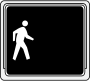
\includegraphics{MUTCD_Ped_Signal_-_Walk}}
           {\caption{Proceed into the intersection}}
\end{figure}

\begin{figure}[H]
  \fcapside
           {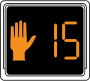
\includegraphics{MUTCD_Ped_Signal_-_Hand_with_timer}}
           {\caption{The walk condition will end in the indicated
               number of seconds.  Do not enter the intersection
               unless you can cross before the condition ends.}}
\end{figure}

\begin{figure}[H]
  \fcapside
           {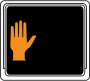
\includegraphics{MUTCD_Ped_Signal_-_Steady_hand}}
           {\caption{Do not enter the intersection.}}
\end{figure}

\newcolumntype{P}[1]{>{\centering\arraybackslash}p{#1}}
\newcolumntype{M}[1]{>{\centering\arraybackslash}m{#1}}
\newcolumntype{L}{>{\centering\arraybackslash}l}

These symbols may be accompanied by audible or tactile signals for
pedestrians with poor sight.

A pedestrian crossing is equipped with a button so the pedestrian can
signal his desire to cross the street.

\subsection{Intersection}
For purposes of illustration, we will consider the following intersection:

\begin{figure}[H]
  {\begin{tikzpicture}
    % road edges
    % southwest edge
    \draw (0.0, 4.8) -- (1.0, 4.8) -- (2.0, 4.4) -- (3.0, 4.4)
    arc [start angle=90, end angle=0, x radius=1, y radius=1] -- (4.0, 0.0);

    % northwest edge
    \draw (0.0, 5.6) -- (3.0, 5.6) arc [start angle=-90, end angle=0,
      x radius=1, y radius=1] -- (4.0, 10.0);

    % southeast edge
    \draw (10.0, 4.6) -- (7.0, 4.6) arc [start angle=90, end angle=180,
      x radius=1, y radius=1] -- (6.0, 0.0);

    % northeast edge
    \draw (10.0, 5.4) -- (7.0, 5.4) arc [start angle=270, end angle=180,
      x radius=1, y radius=1] -- (6.0, 10.0);

    % lanes and medians
    % west side
    \node[anchor=east] at (3.5, 5.4) {6};
    \draw (0.0, 5.2) -- (3.5, 5.2);
    \node[anchor=east] at (3.5, 5.0) {H};
    \draw (2.0, 4.8) -- (3.5, 4.8);
    \node[anchor=east] at (3.5, 4.6) {J};

    % east side
    \node[anchor=west] at (6.5, 4.8) {3};
    \draw (10.0, 5.0) -- (6.5, 5.0);
    \node[anchor=west] at (6.5, 5.2) {D};
    
    % north side
    \node[anchor=south] at (5.8, 6.5) {4};
    \draw (5.6, 10.0) -- (5.6, 6.5);
    \node[anchor=south] at (5.4, 6.5) {5};
    \filldraw (5.2, 10.0) -- (5.2, 6.5) -- (5.15, 6.5) -- (5.15, 8.0) --
    (4.8, 9.0) -- (4.8, 10.0) -- (5.2, 10.0);
    \node[anchor=south] at (4.975, 6.5) {E};
    \draw (4.8, 8.0) -- (4.8, 6.5);
    \node[anchor=south] at (4.6, 6.5) {F};
    \draw (4.4, 10.0) -- (4.4, 6.5);
    \node[anchor=south] at (4.15, 6.5) {G};
    \draw[dashed] (3.75, 6.5) -- (6.25, 6.5) -- (6.25, 6.25) -- (3.75, 6.25) --
    (3.75, 6.5);
    \node[anchor=north] at (5.2, 6.25) {pn};

    % south side
    \node[anchor=north] at (4.2, 3.5) {1};
    \draw (4.4, 0.0) -- (4.4, 3.5);
    \node[anchor=north] at (4.6, 3.5) {2};
    \filldraw (4.8, 0.0) -- (4.8, 3.5) -- (4.85, 3.5) -- (4.85, 2.0) --
    (5.2, 1.0) -- (5.2, 0.0) -- (4.8, 0.0);
    \node[anchor=north] at (5.025, 3.5) {A};
    \draw (5.2, 2.0) -- (5.2, 3.5);
    \node[anchor=north] at (5.4, 3.5) {B};
    \draw (5.6, 0.0) -- (5.6, 3.5);
    \node[anchor=north] at (5.8, 3.5) {C};
    \draw[dashed] (3.75, 3.5) -- (6.25, 3.5) -- (6.25, 3.75) -- (3.75, 3.75) --
    (3.75, 3.5);
    \node[anchor=south] at (5.2, 3.75) {ps};
    
  \end{tikzpicture}}
  {\caption{example intersection}}
\end{figure}

In the diagram above, the north-south boulevard has two lanes in each
direction plus a median which turns into a left turn lane approaching
the intersection.  The two side roads have one or two lanes entering
the intersection and one lane leaving.

Vehicles drive on the right so the nine lanes entering the intersection are
marked with letters A through J, and the six lanes exiting the intersection are
marked with digits 1 through 6.

In the boulevard lanes A and E are left turn lanes, B and F are straight
through lanes, vehicles in lanes C or G may turn right or go straight through.
Right turn on read is permitted from lanes C, D, and G, but not H or J.

A vehicle coming from the west chooses lane H if it wishes to turn left
or go straight, and lane J if it wishes to turn right.
A vehicle coming from the east will be in lane D, from which it can turn
left, turn right, or go straight through.

Each incoming lane is controlled by a signal face and has a sensor that will
notice the presence of a vehicle approaching or waiting in this lane
at the intersection.
The traffic control signal allows traffic to attempt to turn left even
when there is oncoming traffic provided there are no pedestrians on the near
side of the intersection and no cross-traffic.
Straight across traffic is allowed only when
cross traffic is stopped and there are no pedestrians crossing on either side.
U turns are allowed where left turns are allowed.

The two pedestrian crossings are marked in the diagram with dashed lines
and annotated as pn and ps.
A pedestrian is permitted to cross only when there is no vehicle traffic
moving through the crosswalk.

The traffic control signal can sense the approach or presence of an emergency
vehicle but not always which direction it is coming from.
When an emergency vehicle is sensed all traffic is stopped.
However, if the direction of the emergency vehicle can be determined,
traffic is allowed to clear the approach lane.

\section{The Problem}
With that background the problem can be stated simply: operate the traffic
signals so that vehicles and pedestrians can move through
the intersection safely and efficiently.

A vehicle or pedestrian is safe if its journey through the intersection
does not encounter another vehicle.  The movements are efficient if the
average wait of a vehicle or pedestrian at a traffic light is minimized.

In addition, the maximum wait time cannot be excessive: pedestrians and
vehicle operators must be confident that if they wait for a green signal
they will be able to resume their journey without too much delay, or
else they will ignore the signals.

\section{The Solution}
For purposes of exposition, the algorithm that controls the traffic
signals will be broken up into parts that interact with each other
in simple ways.

\subsection{Finite State Machines}
Since each signal face reacts to its environment in similar ways,
we will have a finite state machine for each signal face.
To make the states of the finite state machines clearer we divide them into
two parts: the major states and the minor states within the major states.

The major states are Red,
Yellow and Green, and there are substates within each state.  In addition
each finite state machine has timers and toggles.
A toggle can be true or false,
it can be tested and its value set or cleared.
When we speak of ``setting'' a toggle
that means making it true, whereas ``clearing'' a toggle makes it false.
The vehicle sensors and the desire of a pedestrian
to cross the street are presented to the finite state machines as toggles.
Once set by
the external activity the toggle remains set until the finite state machine
clears it, though if a vehicle is waiting to enter the
intersection or a pedestrian is holding down his button its toggle will
remain true.

When a signal face's finite state machine enters a particular substate
there are actions
which are executed.  While it is in that substate there are conditions
that will cause it to exit the substate and enter another.

\subsection{Travel Paths}
To see how some lanes must be stopped so that others can go, we describe
the intersection in terms of travel paths.  A vehicle approaching the
intersection along a particular lane will exit the intersection on a
different lane; for example the travel path B5 means that the vehicle enters
the intersection on lane B and exits on lane 5.
A line connecting those two lanes is the vehicle's
travel path.

For pedestrians, the travel paths are from the east or west
side of the crosswalk to the other side.  We call the corners
psw, pse, pnw, and pne.  The travel paths are therefore pswpse, psepsw,
pnwpne, and pnepnw.

When two travel paths cross we say that the travel paths conflict.
When that happens only one of the travel paths may have a green light.
Since the traffic control signal only controls whether or not a vehicle
may enter the intersection on a particular lane, and not which
lane it exits on, we can group the travel paths together by entry lane, as
follows:

\begin{longtable}{l |l| p{8cm}}
  \caption{Travel Path Conflicts} \\
  in & out & conflicts with \endfirsthead
  \caption{Travel Path Conflicts continued} \\
  in & out & conflicts with \endhead
  \hline
  A & 6, 2, 1 & D6, D1, D2, F2, G1, G6, H5, H4, H3, J1, psw, pse \\
  B & 5 & D2, D1, D6, E5, E3, H5, H4, H3, psw, pse, pnw, pne \\
  C & 3, 4 & D1, D2, D3, D4, D6, E4, H4, H3, psw, pse, pnw, pne \\
  D & 3, 4, 5, 6, 1, 2 & A2, A1, A6, B5, C4, C3, E3, E4, E5, F2, G1, G6, H3,
  H4, H5, J1, J2, pnw, pne, psw, pse \\
  E & 5, 4, 3 & B5, C4, D2, D1, D6, D4, H5, H4, pnw, pne  \\
  F & 2 & A2, A1, A6, D1, D2, D6, H4, H4, H3, J2, pnw, pne, psw, pse \\
  G & 6, 1 & A6, A1, A2, D2, D1, D6, H5, H4, H3, J1, pnw, pne, psw, pse \\
  H & 5, 4 & A6, B5, C4, D4, D6, D1, D2, E3, E5, E4, F2, G1, pnw, pne \\
  J & 1, 2 & A1, A2, D2, D1, F2, G1, pse, psw \\
\end{longtable}

Since, again, the traffic control signal only controls entry to the
intersection,
we can further simplify the travel path conflict table into a signal face
conflict table and add the pedestrian crosswalks as follows:

\begin{longtable}{c | l}
  \caption{Signal Face Conflict Table} \\
  signal face & conflicts with signal faces \endfirsthead
  \caption{Signal Face Conflict Table continued} \\
  signal face & conflicts with signal faces \endhead
  \hline
  A & pse, psw, D, F, G, H, J \\
  pse and psw & A, B, C, D, F, G, J \\
  B and C & pse, psw, D, E, pne, pnw, H \\
  D & A, pse, psw, B, C, E, pne, pnw, F, G, H, J \\
  E & B, C, D, pne, pnw, H \\
  pne and pnw & B, C, D, E, F, G, H \\
  F and G & A, pse, psw, D, pne, pnw, , H, J \\
  H & A, B, C, D, E, pne, pnw, F, G \\
  J & A, pse, psw, D, F, G \\
\end{longtable}

We also need a table named Partial Signal Face Conflicts.  It is the same
as Signal Face Conflicts except for signal face A which omits F and G,
and signal face E which omits B and C.  This is used for permissive
left turns.

These two tables are specified by the traffic signal engineer
based on the geometry of the intersection.

\subsection{Timers}

Each signal face finite state machine has a set of timers.
A timer is either stopped, running
or completed.  A signal face may start a timer, which takes it from
whatever state it is in to running.  A timer runs for its defined duration,
when it becomes completed.  A signal face may test a timer to see if
it has completed.  If a timer is running when a signal face starts it,
the timer restarts from its beginning.

If a timer has infinite duration, a signal face may start it but
it never reaches completion.

When the traffic control signal is being designed the traffic signal engineer
specifies
the duration of the timers based on the expected traffic speed and volume on
each lane and on the geometry of the intersection.

Here is the list of timers, with the values chosen for each signal face in
our example intersection:

\subsubsection{Green Limit Time}
If we have been green for Green Limit time, we turn red even if there is
no conflicting traffic.

In our example, signal faces B, C, F, and G have their Green Limit times
set to infinity, since these lanes should remain green even in the absence
of traffic.  Signal faces A, D, E, H, J and the pedestrian signal faces
have their Green Limit times set to 60 seconds.

\subsubsection{Left Flashing Yellow Waiting Time}
Lanes A and E will allow a left turn in the presence of oncoming traffic,
called a permissive left turn.
However, if oncoming traffic is heavy enough that a waiting vehicle
cannot make its turn for Left Flashing Yellow Waiting time, the oncoming
traffic will be stopped, thus allowing a protected left turn.

In our example, signal faces A and E have a Left Flashing Yellow Waiting time
of 15 seconds.  The other signal faces do not make use of this timer
since their Signal Face Conflict and Partial Signal Face
Conflict tables are the same.

\subsubsection{Maximum Green time}
If there is no traffic gap for Maximum Green time, and there is conflicting
traffic waiting for us to turn red, turn red anyway.

In our example, signal faces B, C, F, and G have their Maximum Green
times set to 60 seconds; signal faces A, D, E, H, and J to 30 seconds;
and the pedestrian signal faces to 7 seconds.

\subsubsection{Minimum Green time}
When a signal face turns green we want to give the traffic some time
to get moving before we consider turning red.  For pedestrian crossings
this is the Walk time: the time that the signal face displays the walking
person so that the pedestrian can cross the street.

In our example, signal faces B, C, F, and G have their Minimum Green
times set to 10 seconds; signal faces A, D, E, H, and J to 5 seconds;
and the pedestrian signal faces to 7 seconds.

\subsubsection{Minimum Left Flashing Yellow time}
Lanes A and E will allow a left turn in the presence of oncoming traffic,
called a permissive left turn.  Once we have turned on the left flashing
yellow light, we keep it on at least Minimum Left Flashing Yellow time
to make sure the left turning traffic is able to start up.

In our example, signal Faces A and E have their Minimum Left Flashing Yellow
time set to 5 seconds.  The other signal faces do not use this timer
since their SIgnal Face Conflict and Partial Signal Face Conflict
tables are the same.

\subsubsection{Passage Time}
After the minimum green time has elapsed, if there is conflicting traffic
waiting for us to turn red we would like to wait for a gap in our traffic
before turning red.
The Passage time is the length of a gap in our traffic that will permit us
to turn red.

In our example, signal faces A, D, E, H and J have their Passage times
set to 2.3 seconds; signal faces B, C, F, and G to 2.6 seconds; and
the pedestrian signal faces to 0, disabling gap detection
for pedestrians.

\subsubsection{Red Clearance Time}
An important characteristic of any intersection is the time required
for vehicles to move clear of any conflicting travel paths.
The Red Clearance time is the time between when a signal face turns red
and the last vehicle to enter the intersection from that lane has left the
intersection, so that a conflicting travel path can be given a green light.

In our example, signal faces A, D, E, H, and J have their Red Clearance
times set to 1.5 seconds; and signal faces B, C, F, G and the pesestrian
signal faces to 0.4 seconds.

\subsubsection{Red Limit Time}
If we have been red for Red Limit time, we turn green even if there is
no traffic.

In our example, signal faces A, D, E, H, J and all the pedestrian
signal faces have their
Red Limit times set to infinity since those signal faces should
remain red in the absence of traffic.
Signal faces B, C, F, and G have their Red Limit times set to 60 seconds.

\subsubsection{Traffic Still Present}
If we are trying to turn green due to a vehicle being present or approaching
the intersection, but after this much time the vehicle is not present, then
we stop trying to turn green.  The vehicle has likely made a permissive right
turn so there is no longer a need to stop the cross traffic.

In our example, signal faces A, B, C, E, F and G have their Traffic Still
Present timeers set to 10.0 seconds, so a vehicle has time to reach
the Traffic Present sensor after being detected by the Traffic Approaching
sensor.  Signal faces D, H, and J have the timer duration set to 3.0 seconds,
since they don't have a Traffic Approaching sensor. The pedestrian signal
faces are triggered by push buttons, so they cannot sense whether or not
a pedestrian is still present, to they have the timer duration set to
infinity.

\subsubsection{Yellow Change Time}
To give traffic warning that we are soon turning red, we first turn our light
yellow for Yellow Change time.  For pedestrian crossings this is the
Flashing Don't Walk time: the time that the signal face displays the flashing
raised hand and the countdown to encourage the pedestrian to complete
crossing the street.

In our example, signal faces A, B, C, E, F, and G have their Yellow Change
times set to 4.3 seconds; signal faces D, H, and J to 3.0 seconds;
and the pedestrian signal faces to 15.0 seconds.

\subsection{Toggles}

Each signal face finite state machine has a set of togggles which it uses
to control its internal transitions and communicate with the
outside world.  These are:

\subsubsection{Clearance Requested}

A signal face will set Clearance Requested in conflicting signal faces
when it wants the conflicting signal face to turn red so it can turn green.
When a signal face sees that its own Clearance Requested toggle has been
set, it turns red.

\subsubsection{Cleared}

When a signal face has been red long enough for all of its traffic
to have cleared the intersection it sets the Cleared toggle.
This allows conflicting signal faces to turn green.

\subsubsection{Conflicting Paths are Clear}

When a signal face sees this toggle set it can change from circular red
to green, from left arrow red to left arrow green, or from flashing
left arrow yellow to left arrow green.
In the latter case the transition is from permissive left turn to
protected left turn.

\subsubsection{Flash Red}

When a malfunction or an operator sets this toggle, the signal face
will set its light to flashing circular red.

\subsubsection{Flash Yellow}

When a malfunction or an operator sets this toggle, the signal face
will set its light to flashing circular yellow.

\subsubsection{Green Request Granted}

When a signal face sees this toggle set it can start to clear conflicting
paths so it can turn green.

\subsubsection{Manual Green}

When an operator or a central controller sets this toggle,
the signal face will proceed
expediciously through its regular sequence until it can set its light to
green, then remain there.

\subsubsection{Manual Red}

When an operator sets this toggle, the signal face will proceed
expediciously through its sequence until it can set its light to
red, then remain there.

\subsubsection{Partial Conflicting Paths are Clear}

When a signal face sees this toggle set and Conflicting Paths are Clear
not set, it can switch its light from left arrow red to flashing left arrow
yellow, thus allowing permissive left turns.

\subsubsection{Preempt Green}

This toggle is set by an emergency vehicle approaching the intersection
in the lane controlled by this signal face.  The signal face will proceed
expediciously through its sequence until it can set its light to
green, thus making way for the emergency vehicle.

\subsubsection{Preempt Red}

This toggle is set by an emergency vehicle approaching the intersection
but not in the lane controlled by this signal face.
The signal face will proceed expediciously through its sequence until it can
set its light to red, thus preventing
conflicting traffic from interfering with the emergency vehicle.

\subsubsection{Request Clearance}

When a signal face has permission to turn green it sets the Request Clearance
toggle to ask all conflicting signal faces to turn red.

\subsubsection{Request Green Granted}

When a signal face has requested permission to turn green, this toggle
tells it that it has permission.

\subsubsection{Request Green}

When a signal face is red and is preventing traffic from entering the
intersection, it sets toggle Request Green to ask permission to turn green.

\subsubsection{Request Partial Clearance}

When a signal face has permission to turn green, it sets the Request Partial
Clearance toggle to ask that all conflicting signal faces except
those controlling oncoming traffic for left turns turn red.

\subsubsection{Traffic Approaching}

This toggle is set by a sensor some distance from the intersection.
It detects a vehicle approaching from far enough away that if the
signal face turns yellow just before the vehicle triggers the sensor
it will have time to stop safely.
The toggle, once triggered by the sensor, remains set until cleared
by the signal face.

In our example, signal faces A and E have their Traffic Approaching
sensors set at the entrance to the left turn lane.  Signal faces
B, C, F, and G have their sensors set at the edge of the diagram.
Signal faces D, H, J and the pedestrian signal faces do not have traffic
approaching sensors,
so their toggles are set by the Traffic Present sensor.

\subsubsection{Traffic Flowing}

When a signal face is allowing traffic to enter the intersection, either
because it is green or because it is flashing left yellow, it sets this
toggle.  This allows conflicting signal faces who are preventing traffic
from entering the intersection to begin the process of turning green.

\subsubsection{Traffic Present}

This toggle is set by a sensor just before the intersection which detects
traffic controlled by this signal face.
The toggle, once set by the sensor,  remains set until it is cleared
by the signal face.

\subsection{States and Their Transitions}

The signal traffic face finite state machine has three major states,
and each major state has several minor states.

\subsubsection{Red}
The Red major state shows a red light, which means traffic in this
lane must stop.  When the traffic light has been red for Red Clearance Time,
the finite state machine sets its Cleared toggle, which is tested by other
signal faces to see if they can turn green.  If a vehicle or
pedestrian arrives at this signal face it starts the process
of turning green.

Here are the details of the Red state:
      
\input{red_state_table.tex}

\subsubsection{Green}
The Green major state shows a green light, which means traffic in this lane
may proceed through the intersection.  We keep the light green long enough
for the traffic to get moving, then if another signal wants us to turn
red we wait for a break in the traffic.  If there is no break in the
traffic for a while we turn red anyway.  If an emergency vehicle is present
we turn red as quickly as we safely can.

\input{green_state_table.tex}

\subsubsection{Yellow}
The Yellow state is an intermediate state between green and red, and when
flashing means that there may be conflicting traffic.  On left turn signal
faces with a fourth light that shows a flashing yellow left arrow, that
light is included in the Yellow state.

\input{yellow_state_table.tex}

The State Diagram Summary in figure \ref{fig:State_Diagram_Summary}
summarizes the most significant states, substates and
transitions of the finite state machines:

\begin{figure}[htb]
  {\includegraphics{state_diagram}}
  {\caption{State Diagram Summary}\label{fig:State_Diagram_Summary}}
\end{figure}

\subsection{System Programs}

Communication between traffic signal face finite state machiness is handled by
system programs.
These system programs run constantly, reacting to toggles in the
signal faces by setting toggles in other signal faces.

\subsubsection{Green Request Granted}

To prevent two signal faces from bouncing green time between each other,
locking out a third signal face, this system program makes sure that
traffic never has to wait too long for a green light.

This system program maintains a persistent list of signal faces that are
requesting green,
a list of signal faces that are allowed to turn green and a list of signal
faces that have turned green since the currently waiting signal face
has had its chance.
All of these lists start empty.

Go through all of the signal faces looking for those with toggle Request
Green true.  Add each such signal face to the list of
signal faces that are requesting green, unless the signal face is already on
the list or in the set of signal faces allowed to turn green.

If the list of signal faces allowed to turn green is empty, move the
oldest signal face on the list of signal faces that are requesting
green to the list of signal faces allowed to turn green and empty the list
of signal faces that have turned green since the currently waiting
signal face has had its chance.

Although we wish to allow the signal face that has been on the
signal faces requesting to turn green list the longest to turn green
as soon as possible, we can let other signal faces turn green
at the same time or sooner if they will not delay this signal face
from turning green.

If the oldest signal face on the list of signal faces that are
requesting to turn green does not conflict with any of the signal
faces that are already allowed to turn green, move it from the
list of signal faces that are requesting to turn green to the list
of signal faces that are allowed to turn green and empty the list
of signal faces that have turned green since the currently waiting
signal face has had its chance.

Keep doing the above until the list is empty or the oldest signal
face on the list cannot move because of a conflict.

Now we try to let some signal faces turn green out of order, being
careful not to allow a signal face to be starved out of any
opportunity to turn green.

Provided the oldest signal face on the list of signal faces
waiting to requesting to turn green has not been waiting too long,
go through the list of signal faces that are requesting to turn green
starting with the oldest.  For each such signal face that does not
conflict with any of the signal faces already in the set of signal
faces allowed to turn green, and is not in the list of signal faces
that have turned green since the currently waiting signal face has
had its chance, move that signal face to the list of signal faces
allowed to turn green and add it to the list of signal faces that have
turned green since the currently waiting signal face has had its
chance.

Go through the list of signal faces allowed to turn green.  For any
for which toggle Traffic Flowing is true, remove them from the set
since they have now turned green.

Go through the list of signal faces allowed to turn green.  For each
such signal face, set its Green Request Granted toggle, telling it
that it can now turn green.

\subsubsection{Clearance Requested}

When a signal face wants to turn green, it must wait for all conflicting
signal faces to become clear.  This system program conveys the request
for clearance to the necessary signal faces.

Go through all of the signal faces looking for those with toggle
Request Clearance true.  For each such signal face, consult the traffic
signal conflict table to see which signal faces conflict with this one.
For each such signal face, set its Clearance Requested toggle.

\subsubsection{Partial Clearance Requested}

Go through all of the signal faces looking for those with toggle
Request Partial Clearance true.  For each such signal face, consult the
partial signal face conflict table to see which signal faces conflict
with this one.
For each such signal face, set its Clearance Requested toggle.

This is the same as Clearance Requested, but we use the partial signal face
conflict table, which matches the signal face conflict table except
for the left turn lanes, where their conflict with oncoming traffic is
omitted.
This lets left turners try to make a
permissive left turn, but if they cannot the oncoming traffic will also
be stopped.

In our example, the partial signal face conflict table
has signal face A not conflicting with F and G, and E not
conflicting with B and C.  

\subsubsection{Conflicting Paths are Clear}

Go through the signal faces looking for those with toggle Request Clearance
or toggle Request Partial Clearance
true.  For each such signal face, consult the signal face conflict table
to determine which signal faces conflict with this one.  If all of those
signal faces have their Cleared toggles true, set the Conflicting Paths
are Clear toggle in this signal face.

\subsubsection{Partial Conflicting Paths are Clear}

Go through the signal faces looking for those with toggle Request Partial
Clearance true.  For each such signal face, consult the partial
signal face conflict table to determine which signal faces conflict
with this one.  If all of those signal faces have their Clear toggles
true, set the Partial Conflicting Paths are Clear toggle in this
signal face.

\subsubsection{Safety Check}

An error in the description of the finite state machine, or an error
in the implementation of the finite state machine driver or the
system programs may cause the signal faces to get into unintended
states, such that intersecting traffic flows are permitted in the
intersection.  Sucn a condition is unsafe.  Check for incompatible
states and, if such a state is found, set the intersection to flashing.

\section{Wiring the Finite State Machines to the Lamps}

Each signal face finite state machine is wired to the lamps that
it controls.  This lets us use arrow lamps instead of circular lamps
to indicate to the motorist which travel paths are available to him.
In our example, signal face A has its Steady Circular Red output
connected to a lamp which shows a Steady Left Arrow Red.
Table \ref{lamp_wiring} shows wiring between the signal face finite state
machines and the lamps in the signal faces.

\input {lamp_map_names.tex}

\section{Wiring the Finite State Machines to the Sensors}

Each signal face finite state machine is wired to the sensors
for its lane.  The finite state machine expects two sensors:
a distant sensor that warns of an approaching vehicle and
one right at the intersection that senses a vehicle about
to enter the intersection or stopped waiting for the light
to turn green.

In our example, lanes A and E have their distant sensor where
the left turn lane begins; lanes B, C, E, and F have their
distant sensors far enough from the intersection that a vehicle
moving at the speed limit which sees the lamp turn yellow
just as he trips the sensor has time to stop safely.

Lanes D, H, and J do not have distant sensors, so the output
of the near sensor is used for both functions.  The sensors
for the pedestrian signal faces are the button that the pedestrian presses
to cross.

The driving public is accustomed to signal faces which control
adjacent through lanes operating together: they would think it strange
if signal face B turned red while C remained green.  We accomodate this
by connecting the sensors for lanes B and C to both signal face B
and C, and likewise for F and G.

Similarly, if pedestrians can cross the crosswalk in one direction,
it is customary to also allow crossing in the opposite direction,
even if the sensor has not been triggered.  Thus we connect the sensors
for lanes psw and pse to both signal faces psw and pse, and the sensors
for lanes pnw and pne to both signal faces pnw and pne.

\input {sensor_map.tex}

\section{Scenarios}

To illustrate how the above logic causes the signal faces to react
appropriately, I will describe several scenarios using our example
intersection.

\subsection{Idle}

When the intersection starts up all toggles are set to false,
all timers are set to stopped, and each signal face finite state machine
is set to state Red substate Waiting for Clearance.

Each signal face will proceed
from state Red substate Waiting for Clearance to substate Travel Path is Clear
in less than 2 seconds.
If there is no traffic, signals faces A, D, E, H, J and the pedestrian
signal faces will remain red
since their Red Limit timers have an infinite duration, so they will never
complete.
Signal faces B, C, F, and G will proceed to substate Going Green 1 when
their Red Limit timers complete after 60 seconds.

In substate Going Green 1, system program Green Request Granted will notice
that signal faces B, C, F, and G have their Request Green toggles true.
The system program will place all four signal faces on its list of traffic
signals requesting to turn green.  It will move one of them to the list
of signal faces allowed to turn green.  Assume it is signal face B.
It will then go through the three
remaining signal faces and discover that signal face C does not have
a conflict with B and so move it to the set of signal faces allowed
to turn green.  Similarly, signal face F has no conflict with B or C,
and G has no conflict with B, C, or F, so we end up with B, C, F and G
on the list of signal faces allowed to turn green.

Signal faces B, C, F, and G will proceed to state Red
substate Going Green 2 where they will set toggle Request Partial Clearance.

System Program Partial Clearance Requested will notice that signal faces
B, C, F, and G have Request Partial Clearance true,
and will consider setting toggle Clearance
Requested in signal faces D, E, H, J, and the pedestrian signal faces.
However, those signal faces
are in state Red substate Travel Path is Clear so they all have their
Cleared toggles set.

The Partial Conflicting Paths are Clear system program will notice that the
signal faces that partially conflict with B, C, F, and G are clear,
so will set the
Partial Conflicting Paths are Clear toggle in signal faces B, F, F, and G.
Similarly, the Conflicting Paths are Clear system program will set
the Conflicting Paths are Clear toggle in those same signal faces.

Signal faces B, C, F, and G will proceed from state Red substate
Going Green 2 to state Green substate Minimum Green.
This will cause those signal faces to turn green and set toggle
Traffic Flowing.

System program Green Request Granted will notice that signal faces
B, C, F, and G have their Traffic Flowing toggle true,
and so will remove them from the list of signal faces allowed to turn green.
This will cause the list to be empty.

The net effect is that after 60 seconds signal faces
B, C, F, and G turn green.  Because the Green Limit timer duration for signal
faces B, C, F, and G are infinity they will remain green unless
a conflicting signal face needs to turn green.  Because the Red Limit
timer duration for the other signal faces is infinite they will stay red
unless some traffic appears on their lanes.

We will call this situation, with signal faces B, C, F, and G green
and the others red and clear the idle condition, since it will persist
in the absence of traffic.

This table of events details the progression from power on to the idle state.

\input{idle_table.tex}

\subsection{Pedestrian Crossing on South Side of Intersection}
A pedestrian who wishes to cross the boulevard on the south side
presses his button.  Assuming we are in the idle condition
with signal faces
B, C, F and G green and A, D, E, H, J, and the pedestrian signal faces
red and clear.

Signal faces psw and pse will proceed to substate Going Green 1 where
they will set
toggle Request Green.  The Request Green Granted system program will act
as described above to set the Request Green Granted toggle since no other
signal faces are waiting to turn green.  Signal faces psw and pse will then
proceed to substate Going Green 2 where they will set toggle Request Partial
Clearance.  System program Partial Conflicting Paths are Clear will set
the Clearance Requested toggles in signal faces B, C, F, and G,
but not in signal faces A, D and J because they are aleady clear.
Signal faces B, C, F, and G are in state Green substate Waiting for Clearance
Request because their Green Limit timer has a duration of infinity and
they have seen no recent traffic.

Signal faces B, C, F and G will enter state Yellow substate Going Red.
When their Yellow Change timers complete they will proceed to state Red
substate Waiting for Clearance.
When their Red Clearance timers complete they will go
to substate Travel Path is Clear and set toggle Cleared.

The Conflicting Paths are Clear system program will notice that
signal faces A, B, C, D, F, G, and J are all clear and set the
Conflicting Paths are Clear toggle in signal faces psw amd pse.  Similarly,
the Partial Conflicting Paths are Clear system program will set the
Partial Conflicting Paths are Clear toggle.

Signal faces psw and pse will transition to state Green substate Minimum Green.
This will cause the pedestrian signs to display a walking man, the equivalent
of green.  Assuming there is no other traffic, signal faces pse and psw
will remain green
until the Red Limit timers complete on signal faces B, C, F, and G.
This will cause signal faces pse and psw to follow the progression described
above
for signal paths B, C, F, and G.  Signal faces pse and psw will transition
to state Yellow
substate Going Red, where they will display the hand with a countdown timer
showing how many seconds are left in the Yellow Change timer.  When the Yellow
Change timer is complete signal faces psw and pse will transition to the
Red state,
substate Waiting for Clearance.  When their Red Clearance timers completes
they will
transition to substate Travel Path is Clear and set the Cleared toggle.

Signal faces B, C, F, and G will then proceed as described above
in the Idle scenario to turn green.

The following describes the events in detail.

\input{pedestrian_table.tex}

\subsection{Left Turn}

A vehicle arrives at Signal Face A.  Assume we are in the idle condition
with signal faces B, C, F, and G green and the others red and clear.

Signal face A requests permission to turn green, which it receives right
away because no other signal face is requesting permisison to turn green.

Signal face A then causes the Partial Clearance Requested system program
to set the Clearance Requested toggle in signal faces psw, pse, D, H, and J.

Signal faces psw, pse, D, H, and J are already clear, so system program Partial
Conflicting Paths are Clear sets toggle Partial Conflicting Paths are Clear
in signal face A.
Notice that signal faces F and G are not clear, so toggle Conflicting Paths
are Clear does not get set in signal face A.

Signal face A proceeds to state Yellow substate Flashing 1.  The red light
at lane A turns to a yellow flashing light, telling the vehicle operator
that he may turn left but must watch for oncoming traffic.

When the Left Flashing Yellow Waiting timer completes, if there is still
traffic for
signal face A it proceeds to substate Going Green where it sets the
toggle Request Clearance, causing system program Clearance Requested to
set the Clearance Requested toggle in signal faces psw, pse, D, F, G, H, and J.

Signal faces psw, pse, D, H and J are already clear.  Signal faces F and G turn
yellow, then red, then become clear.

When signal faces F and G become clear system program Conflicting Paths
are Clear will set the Conflicting Paths are Clear toggle in signal face
A which will cause signal face A to turn green.

When the Green Limit timer in signal face A completes, signal face
A will turn red and eventually become clear, which will allow
signal faces F and G to turn green when their Red Limit timers complete,
as described above.

The following events take place assuming that the driver of the
car turning left is not willing to make the permissive turn,
and so waits for the green arrow.

\input{left_turn_delayed_table.tex}

However, if the vehicle makes the permissive left turn, signal face A
returns to red, never causing signal faces F and G to turn red,
as illustrated in the following events.

\input{left_turn_table.tex}

\subsection{Pedestrian and Near Left Turner}

Building upon the previous two scenarios, suppose after the pedestrian
has pushed his button and begun to cross, a vehicle arrives at lane A.
Signal face A will be be given permission to turn green right away, since no
other signal faces are waiting to turn green.  It will then request
that signal faces psw, pse, D, H and J turn red.  Signal faces D and J
will already be clear because signal faces pse and psw is green,
and signal face H has never been green, so signal face A is waiting
only for signal faces psw and pse.

When signal faces psw and pse are clear signal face A will turn green because
signal faces F and G are clear due to signal faces psw and pse,
so the left turn is protected rather than permissive.

Signal faces B, C, F, and G will want to turn green and so signal faces
F and G will ask signal face A to turn red.  Signal faces B and C
will turn green without waiting for signal face A to clear, since
they do not conflict.  When signal face A is clear signal faces
F and G will turn green, getting us back to the idle state.

Here are the events of this scenario, with less detail than
previously.

\input{pedestrian_and_left_turn_table.tex}

\subsection{Multiple Arrivals}

Suppose we are in the Idle condition when traffic arrives in quick succession
at signal faces A, psw, D, E, pne, H, and J in that order.

Signal face A turns left flashing yellow immediately since lanes
F and G are allowing traffic to flow.

Signal face psw asks signal faces A, B, C, F, and G to turn red.
Signal face A is currently left flashing yellow but signal faces
B, C, F, and G turn yellow and then red.

With the through lanes all stopped signal face A turns
green, then yellow, then red, permitting the pedestrians in the south
crosswalk to cross.  Signal face E does the same, permitting the
pedestrians in the north crosswalk to cross.

When the pedestrians in the south crosswalk have crossed, signal
face J turns green.  Similarly, when the pedestrians in the
north crosswalk have crossed, signal face H turns green.

When signal faces H and J have turned red, signal face D
can finally turn green.  When it turns red signal faces
B, C, F, and G turn green, getting us back to the idle state.

To summarize, if traffic arrives in quick succession on signal faces
A, psw, D, E, pne, H and J, traffic will flow through signal faces
A and E, then through psw and pne, then H and J, and finally D.

The following table shows the most significant events in this scenario.

\input{multiple_table.tex}

\subsection{Emergency Vehicle}

The presence of an emergency vehicle preempts the normal flow of traffic
to give priority to the emergency vehicle. The sensor for emergency
vehicles controls two toggles: Preempt Red and Preempt Green.
If the sensor detects an emergency
vehicle it sets the Preempt Red toggle in all signal faces.
However, if it is able to determine from which direction the emergency vehicle
is approaching it instead sets the Preempt Green toggle, as follows:

\begin{longtable}{c | l | l}
  \caption{Emergency Vehicle control} \\
  From Direction & Preempt Red & Preempt Green \endfirsthead
  \caption{Emergency Vehicle Control continued} \\
  From Direction & Preempt Red & Preempt Green \endhead
  \hline West & A, psw, pse, B, C, D, E, pnw, pne, F, G & H, J \\
  \hline South & psw, pse, D, E, pnw, pne, F, G, H, J & A, B, C \\
  \hline East & A, psw, pne, B, C, E, pnw, pne, F, G, H, J & D \\
  \hline North & A, psw, pne, B, C, D, pnw, pne, H, J & E, F, G \\
  \hline
\end{longtable}

\section{Manual Control}

An operator may take manual control of the traffic control signal.
The operator's control panel contains the following controls:

\subsection{Off Switch}
The Off switch turns off power to the traffic control signal and all
of the signal faces.  Turning off power is necessary for safety during
maintenance.

\subsection{Mode}

There is a multi-position mode switch:

\subsubsection{Automatic}

With the mode switch set to Automatic the traffic control signal
receives signals from the sensors and acts appropriately, as described
above.  The operator is an observer who can see the color of each
signal face, the state of the toggle corresponding to each vehicle detector,
and the names of the signal faces in each persistent list maintained by
the Green Request Granted system program.

The operator can choose to also see the state and substate of each signal
face, the state of each timer, the time until completion of each
running timer, and the state of each toggle and sensor.

\subsubsection{Manual}

With the mode switch set to Manual, the traffic control signal is
disconnected from the sensors.  The operator has
a 3-position switch on the display of each lane to cause that lane to turn red
or green.  The Red position sets the Manual
Red toggle and the green position sets the Manual Green toggle.
The third position is neutral, which sets neither toggle.

In this mode, as in Automatic mode, the operator sees the state of
each signal face and each vehicle detector.  Also as in Automatic mode,
the operator can choose to also see the substate of each signal face,
the state of each timer, the time until completion of each running
timer, and the state of each toggle.

In this mode the operator must specify when each signal face turns
red and green.  Notice that all of the safety interlocks still
are in effect: setting a signal face to green while a conflicting
signal face is already set to green will have no effect until the
conflicting signal faces are set to red or neutral.

A manual control console can be either local or remote.  If it is remote
there should be cameras giving a complete picture of the intersection
to the remote operator.

\subsubsection{Flashing}

With the mode switch set to Flashing, signal faces with Red Limit
timers having finite duration have their Flash Yellow toggles set
and all other signal faces have their Flash Red toggles set.

If the traffic signal controller detects a malfunction it switches
to Flashing mode itself.  In addition, if the computer in the traffic
signal controller fails there is hardware in the traffic signal
controller to flash the lights independent of the computer.

\subsubsection{Programming}

This mode is protected so only authorized persons can access it.
It works the same as Automatic mode except the operator is also allowed to
adjust the duration of the timers in each signal face, and update the
Signal Conflict Table and the Partial Signal Conflict Table.

These adjustments can cause unsafe conditions and so should be limited
to highly trusted personnel.

\section{Central Control}

The signaling procedure described here takes only the traffic at a single
intersection into account.  Where there are many intersections close
together it will be worthwhile to control them all as a single system.
In such a control system a central controller will provide overall
coordination while each intersecton operates as described here except as
directed by the central controller.

The algorithm used by the central controller is beyond the scope of this
description, but from the point of view of an individual intersection
the central controller will use the Manual Green toggle to clear paths
through several intersections so that traffic can flow freely in the
chosen directions.

The central controller will be able to see all of the sensors of all
of the intersections it controls.

\section{Traffic Simulation}

In order to test the code before we go to the expense of installing
it in a traffic control signal, we will need a simulator to activate the
traffic present and traffic approaching sensors.  The traffic simulator
for vehicles introduces vehicles at the edge of the diagram and
runs them through the intersection and out again, making sure vehicles
behind stopped vehicles stack up.  Pedestrians just cross the street
without concern about how many can fit in a crosswalk at a time.

The traffic simulator prints information about how the simulated
traffic is proceeding through the intersection, so we can see how
traffic flows.  For context, the signal faces also print information
about the color of each signal face when it changes.

\subsection{Dimensions}

A realistic simulation must be based on the sizes and speeds of real objects.
The sensor placements and timer values for the intersection are then
based on those sizes and speeds.

\begin{description}
\item[Travel Lane Width]{The travel lanes are 12 feet wide.  Note that lanes
  A and E have a 5.5-foot margin separating them from lanes B and F,
  respectively, so that the left turn lanes do not interfere with each other.}
\item[Travel Lane Length]{Travel lanes A and E are 450 feet in length.
  This is 363 feet to stop from 45 miles per hour in a comfortable 11 seconds,
  plus space for five cars or two trucks waiting for the light to change.
  The other travel lanes extend beyond the simulation.}
\item[Car size]{Cars are 15 feet long and 5.8 feet wide}
\item[Truck Size]{Trucks are 40 feet long and 8.5 feet wide.}
\item[Intersection]{The example intersection is 36 feet from north to south
  and 65.5 feet from east to west.}
\item[speed limits]{The speed limit on lanes B, C, D, F, and G is
  45 miles per hour; on lanes A, D, E, H, and J 25 miles per hour,
  on the pedestrian crosswalks, 3.5 feet per second.
  If a vehicle is passing through the intersection it maintains the
  speed limit of its entering lane, but if it has to stop it enters
  the intersection at 25 miles per hour.}
\item[Traffic Approaching Sensors]{The Traffic Approaching sensors are placed
  far enough behind the stop line to give the vehicle operator time to stop
  if the light turns yellow just as the vehicle reaches that point.
  Lanes B, C, F, and G have these sensors 365 feet behind the stop line;
  lanes A, and E have them at the beginning of the lane; the other lines
  do not have them.}
\item[Minimum Green]{The minomum green interval for lanes B, C, F, and G
  is 12 seconds; for lanes D, H, and J 7 seconds; for lanes A and E 5 seconds;
  for the pedestrian lanes 6 seconds.}
\item[Passage Time]{The passage time for lanes B, C, F, and G is 3.5
  seconds; for lanes A, D, E, H, and J is 1.9 seconds;
  for the pedestrian lanes is 1 second.}
\item[Maximum Green]{The maximum green interval for lanes B, C, F, and G
  is 60 seconds; for lanes D, H, and J 40 seconds; for lanes A and E
  20 seconds; for the pedestrian lanes 10 seconds.}
\item[Traffic Still Present]{The traffic still present interval for
  lanes A, B, C, E, F, and G is 10.0 seconds; for lanes D, H, and J is
  3.0 seconds; for the pedestrian lanes is infinity.}
\item[Yellow Change]{The yellow change interval is 5 seconds on lanes
  B, C, F and G; 4 seconds on A and E; 3.5 seconds on lanes D, H and J;
  19 seconds on the pedestrian lanes.}
\item[Red Clearance]{The red clearance interval is 1 second on lanes A, B, C,
  E, F, G and J; 1.5 seconds on lanes D, and G; 3 seconds on
  the pedestrian lanes.}
\end{description}

\section{Licensing}
\label{section:Licensing}
As noted on the first page, this paper is licensed under a Creative
Commons Attribution-ShareAlike 4.0 International License.

The full text of the Creative Commons Attribution-ShareAlike 4.0
International license is at this web site:
\href{https://creativecommons.org/licenses/by-sa/4.0/legalcode}{https://creativecommons.org/licenses/by-sa/4.0/legalcode}%
What follows is a human-readable summary of it.

\subsection{You are free to:}
\begin{description}
\item[Share ---]copy and redistribute the material in any medium or format, and
\item[Adapt ---]remix, transform, and build upon the material
\end{description}
for any purpose, even commercially.  The licensor cannot revoke these
freedoms as long as you follow the license terms.
\subsection{Under the following terms:}
\begin{description}
\item[Attribution ---]You must give appropriate credit\footnote{If supplied,
  you must provide the name of the creator and attribution parties,
  a copyright notice, a license notice, a disclaimer notice, and a link
  to the material.}, provide a link to
  the license, and indicate if changes were made\footnote{You must indicate if
    you modified the material and retain an indication of previous
    modifications.}.  You may do so in any
  reasonable manner, but not in any that suggests the licensor endorses you
  or your use.
\item[ShareAlike ---]If you remix, transform, or build upon the material,
  you must distribute your contributions under the same
  license\footnote{You may also use any of the licenses listed as compatible
    at the following web site:
    \href{https://creativecommons.org/compatiblelicenses}{https://creativecommons.org/compatiblelicenses}}
  as the original.
\item[No additional restrictions ---]You may not apply legal terms or
  technological measures\footnote{The license prohibits application of
    effective technological measures, defined with reference to Article 11
    of the WIPO Copyright Treaty.}
  that legally restrict others from doing anything
  the license permits.
\end{description}
\subsection{Notices:}
\begin{itemize}
\item{You do not have to comply with the license for elements of the
  material in the public domain or where your use is permitted by an
  exception or limitation.}
\item{No warranties are given.  The license may not give you all of the
  permissions necessary for your intended use.  For example, other rights
  such as publicity, privacy or moral rights may limit how you use the
  material.}
\end{itemize}

\bibliography{references}

\end{document}
